\documentclass{inetese}
\usepackage{isolatin1}       %para os acentos iso
\usepackage{graphicx}        %incluir figuras encapsulated postscript
\usepackage{babel}
\usepackage{listings}
%\RequirePackage[dvips]{graphicx}

\ineTitulo{JMinimizer: Um Compactador de Aplica��es Java.}

\ineAutor{Thiago Le�o Moreira}
\ineOrientador{Prof. Dr. Ant�nio Augusto Medeiros Fr�hlich}

\ineAreaConcentracao{Ferramentas de desenvolvimento}
\ineTipoTese{disserta��o}

\ineGrau{Bacharel}
\ineMes{Novembro}
\ineAno{2004}

\ineCoordenadorCurso{Prof. Dr. Jos� Mazzucco Junior}
\ineMembroBancaA{Prof. Dr. Luiz Carlos Zancanella}
\ineMembroBancaB{M. Sc. Tiago Stein D\'Agostini}

\begin{document}

\inePaginaDeRosto
\inePaginaDeAprovacao

\begin{ineEpigrafe}
``A verdadeira fun��o do homem � viver \\
  e n�o apenas existir.''\\
- Jack London
\end{ineEpigrafe}

\begin{ineOferecimento}
  ``A mim, pelas noite n�o dorminadas \\e as baladas perdidas...''
\end{ineOferecimento}

%\begin{ineAgradecimentos}
%  Agradecimentos...
%\end{ineAgradecimentos}

\begin{ineResumo}
O crescente aumento da popularidade da linguagem de programa��o Java levou tamb�m a um aumento, no desenvolvimento de frameworks e bibliotecas utilit�rias, que facilitam o desenvolvimento de aplica��es. No entanto estes frameworks e bibliotecas aumentam o tamanho da aplica��o final, podendo at� ultrapassar em muitas vezes o tamanho da aplica��o que efetivamente resolve o problema de neg�cio. Frameworks e bibliotecas geralmente s�o desenvolvidos para resolver ou tratar de problemas para uma grande quantidade de situa��es. No entanto aplica��es s�o criadas para resolver um problema espec�fico, sendo assim essas aplica��es n�o utilizam todos os recursos que um framework ou uma biblioteca oferecem. � nessas funcionalidades in�teis para a aplica��o espec�fica que o JMinimizer far� e/ou remover� as mesmas.

  \paragraph{Keywords:} Java, J2ME, celular, PDA's.
\end{ineResumo}
                                                                                                                            
\begin{abstract}
  Abstract
  \paragraph{Keywords:} Java, J2ME, celular, PDA's.
\end{abstract}

% Insere o Sum�rio
\tableofcontents    \clearpage
                                                                                                                            
% Insere a lista de Figuras e de Tabelas
\listoffigures \clearpage
\listoftables \clearpage

\chapter{Introdu��o}

Este trabalho consiste do estudo e desenvolvimento de uma aplica��o capaz de analisar uma outra aplica��o Java\cite{java} e apartir dessa analise transformar a aplica��o, de forma que seu comportamante n�o se modifique, tentando reduzir o seu tamanho original.

\section{Motiva��o}
A popularidade da linguagem de programa��o Java\cite{java}, principalmente para pequenos dispositivos\cite{j2me} %COLOCAR AQUI INFO SOBRE A QTD DE CELULARES %
 (celulares, PDA's \footnote{Personal Digital Assistant}, smart phones, etc), resultou num aumento significante de bibliotecas utilit�rias e frameworks que facilitam e aumentam a produtividade no desenvolvimento de aplica��es para esta linguagem. Tais bibliotecas e frameworks s�o utilizados como infra-estrutura na solu��o de problemas espec�ficos.
Bibliotecas para logging, manipula��o de documentos XML, constru��o de interfaces gr�ficas, frameworks para desenvolvimento WEB, para persist�ncia de dados, etc\ldots s�o algumas aplica��es que estas bibliotecas de classes possuem. 
Sites como http://ws.apache.org, http://java.net, http://jakarta.apache.org, http://www.sf.net s�o web sites especializados em abrigar projetos de frameworks e bibliotecas para a linguagem Java\cite{java}, neles s�o disponibilizados dezenas e at� centenas de pequenos e grandes projetos destinados a facilitar o desenvolvimento de aplica��es \cite{java}, sendo ela para qualquer uma das tr�s plataformas: J2ME\footnote{Java 2 Micro Edition}, J2SE\footnote{Java 2 Standard Edition}, J2EE\footnote{Java 2 Enterprise Edition}. Poupando assim tempo e dinheiro de construir e depurar classes de infra-estrutura.
No entanto a utiliza��o de bibliotecas de terceiros pode acarretar num aumento do tamanho da aplica��o se estas bibliotecas n�o tiverem dispon�veis no ambiente de execu��o do aplicativo.
Em conseq��ncia do aumento do tamanho da aplica��o tamb�m aumentar� o tempo para se realizar o download (se for esta a forma de distribui��o do aplicativo) e aumentar� o espa�o necess�rio para acomodar a aplica��o no dispositivo. Este �ltimo � de suma import�ncia quando desenvolvemos aplica��es para a plataforma J2ME\footnote{Java 2 Micro Edition}, onde os dispositivos alvos podem ter somente uma pequena quantidade de espa�o para o armazenamento de aplica��es.
Isto exposto verificamos que a utiliza��o de bibliotecas de terceiros pode resolver o problema de desenvolver e depurar classes para a infra-estrutura e criar outros problemas relacionados ao armazenamento e ao tempo de obten��o da aplica��o. No entanto este segundo, parece ser de mais f�cil solu��o. Uma primeira alternativa de solu��o para o problema seria aumentar a capacidade de armazenamento do aparelho/dispositivo ou adquirir um aparelho/dispositivo similar com maior capacidade de armazenamento. Mas se n�o for poss�vel aumentar a capacidade de armazenamento, nem de trocar de aparelho/dispositivo a segunda solu��o seria tentar retirar do c�digo gerado todo o tipo de informa��o e estrutura que n�o ir� afetar a execu��o normal do aplicativo. E � nesta segunda solu��o que este trabalho de conclus�o de curso � baseado.

\section{Justificativa}

\subsection{Cient�fica}
O desenvolvimento dessa disserta��o contribuir� para a comunidade cient�fica no esclarecimento da estrutura do \textit{bytecode} Java\cite{java} e quais dessas estruturas podem ser removidas.

\subsection{Pessoal}
A grande curiosidade que sempre tive em rela��o ao \textit{bytecode} Java\cite{java}, que � meu instrumento de trabalho, e a necessidade de desenvolver um trabalho de conclus�o de curso para Universidade Federal de Santa Catarina me levaram a desenvolver essa disserta��o.

\subsection{Social}
A possibilidade de desenvolver aplica��es e compartilha-las com meus amigos, sempre foi algo que imaginei um dia fazer e a plataforma J2ME\cite{j2me}, me possibilitou realizar esse desejo. Por esse motivo desenvolvi o JMinimizer, para auxiliar desenvolvedores que como eu desejam distribuir suas aplica��es entre seus amigos.

\section{Objetivos}

\subsection{Geral}
Desenvolver uma ferramenta de desenvolvimento de aplica��es Java\cite{java} que auxilie o \textit{deployment} dessas aplica��es na maior quantidade de dispositivos quem suportam a plataforma J2ME\cite{j2me}
\subsection{Espec�ficos}
Esse projeto apresenta os seguintes objetivos espec�ficos.

\begin{itemize}
\item{Conhecimento}
\begin{itemize}
\item{Consolidar meus conhecimentos na t�cnologia Java\cite{java}.}
\item{Aprender as etapas de desenvolvimento de uma aplica��o open source.}
\end{itemize}
\item{Criar uma ferramenta capaz de diminuir o tamanho de uma aplica��o Java\cite{java}}
\end{itemize}

\chapter{Outras Ferramentas e trabalhos}
Nas pesquisas que desenvolvi pude observar que muitos trabalhos j� foram realizados na busca por uma diminui��o das aplica��es Java\cite{java}. Alguns propondo uma reestrutura��o do bytecode java \cite{tailored}, outros sugerindo uma compacta��o diferente para os arquivos JAR \cite{jar} \cite{jazz}, no entanto estes propoem mudan�as estruturais muito porfundas, tanto nos arquivos class ou jars, t�o profundas que s� ferramentas especiais s�o capazes de ler estes tipos de arquivo. Porem tamb�m encontrei ferramentas que reduzem as aplica��es Java sem modificar sua estrutura b�sica e assim, s�o perfeitamentes compat�veis com a especifica��o Java \cite{javaspec} entre elas est�o o Jax\cite{jax},  SophiaCompression\cite{sophia} entre outras. A seguir ser�o descritas brevemente cada uma das ferramentas que estudei.

\section{Obfuscadores}
Obfuscadores s�o ferramentas de grande utiliza��o na distribui��o de aplica��es Java eles n�o impedem, mas dificultam a engenharia reversa que consiste em a partir do arquivos class obter um arquivo fonte. Al�m de obfuscarem os arquivos class essas ferramentas tem como efeito colateral a diminui��o da aplica��o final, por isso foram objetos de pesquisa dessa tese. Isto ocorre devido a troca dos nomes das classes e pacotes por nomes mais simples e compactos por exemplo, a classe original com nome \textit{net.java.dev.jminimizer.JMinimizer} � renomeada para \textit{a.b.c.d.A}, isto impacta significativamente na diminui��o dos arquivos class.

\subsection{Retroguard}
O Retroguard � um obfuscador de bytecode, uma ferramenta projetada para substituir identificadores e atributos de compreens�o f�cil por humanos por strings sem sentido, tornando a engenharia reversa quase imposs�vel. O resultado da execu��o do Retroguard � aplica��es menores e com o c�digo fonte protegido. Retroguard � distribuido sobre licensa GNU LGPL\footnote{Lesser General Public License}. 
Algumas caracter�sticas:
\begin{enumerate}
\item redu��o do tamanho do bytecode Java (reduzindo 50\% � poss�vel, 20-30\% � t�pico) levando � obten��o mais r�pida das aplica��es 
\item projetado para ser f�cilmente incorporado ao processo de desenvolvimento de aplica�l�es Java.
\item permite uma costumiza��o completa do processo de obfusca��o.
\item suporta multiplos \textit{entry points}.
\item atual sobre arquivos JAR\cite{jar}.
\item obfusca��o � controlado por uma linguagem de script flex�vel.
\item uma interface gr�fica � provida para um simples gerenciamento de scripts.
\item usa massivamente sobrecarga de nomes de m�todos e campos para um aumento da seguran�a.
\item gera unicamente bytecode Java verificado e completamente compat�vel com a especifica��o da m�quina virtual Java.
\item atualiza o arquivo Manifest dos arquivos JAR, utilizanbdo nomes obfuscados e automaticamente gerando menssagens sum�rio MD5 e SHA-1.
\end{enumerate}

\subsection{ProGuard}
ProGuard � um otimizador e um obfuscador para bytecode Java. Ele pode detectar e remover classes, m�todos, campos e atributos que n�o s�o usados. Tamb�m pode otimizar e remover instru��es n�o usadas. Finalmente, ele renomeia classes, campos e m�todos usando nomes curtos e sem sentido, resultando em arquivos JARs menores e de dif�cil execu��o de uma poss�vel engenharia reversa.

\section{Compactadores}
\subsection{SophiaCompress}
\subsection{Jax}
\subsection{Jazz}

\chapter{Fundamenta��o Te�rica}
Para poder realizar as transforma��es que este trabalho se porpo� em fazer � necess�rio antes, uma breve explica��o da estrutura do objeto alvo dessa disserta��o, o bytecode Java.
O produto final do desenvolvimento de uma aplica��o Java � um ou mais arquivos class, tamb�m chamados de bytecode. Cada arquivo com a extens�o class representa uma classe ou interface na aplica��o, tanto um como o outro possuem a mesma estrutura em arquivo, h� somente uma flag diferenciando um do outro. Esses arquivos class s�o o resultado da compila��o dos arquivos de c�digo fonte, e sua estrutura � praticamente um mapeamento um para um da linguagem Java.
� atravez desses arquivos class que foram feitas analises e transforma��es na sua estrutura para reduzir o tamanho das aplica��es Java. 

\section{A estrutura do bytecode}

Cada arquivo com a extens�o class representa uma classe ou uma interface na linguagem Java. Esses arquivos s�o constitu�dos de um array de bytes.
\begin{figure}[ht]
  \centering
  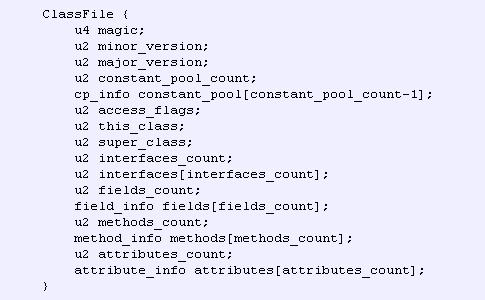
\includegraphics[width=10cm,height=9cm]{imagens/classfile.jpg}
  \caption{formato de um arquivo .class\label{img:classfile}}
\end{figure}

A figura \ref{img:classfile} exemplifica de maneira simples a organiza��o e o significado de cada byte ou conjunto de bytes na estrutura do arquivo class. O significado das representa��es u2 e u4 s�o: u representando um byte sem sinal e o decimal (2 e 4) representado a quantidade de bytes. Por exemplo, o valor magic � composto dos quatros primeiros bytes sem sinais do arquivo class. A seguir ser�o exemplificados cada uma das estruturas que comp�em o bytecode.

\begin{enumerate}
\item magic: este numero � fixo para qualquer bytecode e tem o valor 0xCAFEBABE. O objetivo desse identificador � previnir as JVMs de carregar outras coisas que n�o sejam classes Java.
\item minor\_version: determina a menor vers�o que o bytecode suporta.
\item major\_version: determina a maior vers�o que o bytecode suporta.
\item constant\_pool\_count: determina a quantidade de constantes dispon�veis no pool de constantes.
\item constant\_pool:  estrutura que contem todas as constantes utilizadas no bytecode. Estas constantes podem ser Strings, ints, longs, doubles, etc.
\item access\_flags:  este numero mascara os tipos de acesso que esta classes ou interface pode conter.
\item this\_class:  � o �ndice no pool  de constantes que contem o nome da classe.
\item super\_class: � o �ndice no pool de constantes que contem o nome da super classe.
\item interfaces\_count: determina a quantidade de interfaces que esta classe implementa diretamente, ou o numero de interfaces que esta interface estende.
\item interfaces:  um array contendo �ndices para os nomes das interfaces no pool  de constantes, que este bytecode implementa ou estende.
\item fields\_count: determina a quantidade de campos que esta classe ou interface possui.
\item fields: uma tabela que contem estruturas que representam um campo. A figura \ref{img:field} representa essa estrutura.

\begin{figure}[ht]
  \centering
  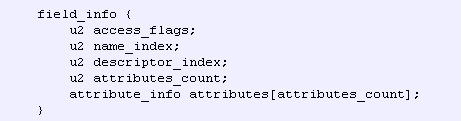
\includegraphics[width=8cm,height=5cm]{imagens/field.jpg}
  \caption{estrutura de um campo \label{img:field}}
\end{figure}

\begin{enumerate}
\item access\_flags:  este numero mascara os tipos de acesso que este campo pode ter.
\item name\_index: �ndice no pool de constantes que contem o nome do campo.
\item descriptor\_index: �ndice no pool de constantes que contem a assinatura do campo.
\item attributes\_count: determina a quantidade de atributos que este campo possui.
\item attributes:  tabela que contem estruturas que representam os atributos deste campo.
\end{enumerate}
\item methods\_count: determina a quantidade de m�todos que esta classe ou interface possui.
\item methods: tabela que contem estruturas que representam um m�todo. A figura \ref{img:method} representa essa estrutura.

\begin{figure}[ht]
  \centering
  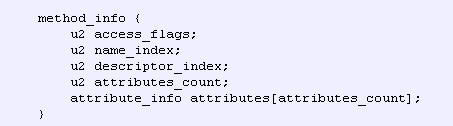
\includegraphics[width=8cm,height=5cm]{imagens/method.jpg}
  \caption{estrutura de um m�todo \label{img:method}}
\end{figure}

\begin{enumerate}
\item access\_flags:  este numero mascara os tipos de acesso que este m�todo pode ter.
\item name\_index: �ndice no pool de constantes que contem o nome do m�todo.
\item descriptor\_index: �ndice no pool de constantes que contem a assinatura do m�todo.
\item attributes\_count: determina a quantidade de atributos que este m�todo possui.
\item attributes:  tabela que contem estruturas que representam os atributos deste m�todo.
\end{enumerate}
\item attributes\_count: determina a quantidade de atributos que esta classe ou interface possui.
\item attributes: tabela que contem estruturas que representam os atributos desta classe ou interface.
\end{enumerate}

Conhecendo a fundo o bytecode foram observadas estruturas que podem receber transforma��es ou at� mesmo serem retiradas, visando a diminui��o do tamanho da aplica��o. Na especifica��o da linguagem Java, exatamente na se��o 4.7 de The JavaTM Virtual Machine Specification\cite[javaspec], est� explicito que algumas das estruturas que encontramos no bytecode podem ser facilmente retiradas sem mudan�a no comportamento do software. Tais estruturas s�o: SourceFile, LineNumberTable e LocalVariableTable, elas representam respectivamente, o nome do arquivo fonte a tabela do n�mero das linhas no c�digo fonte e a tabela de vari�veis locais dos m�todos. V�rios compiladores fornecem meios, atrav�s de parametros, de, na hora da gera��o do bytecode, os atributos respons�veis pela depura��o serem exclu�dos do arquivo class. Esta � uma t�cnica de compacta��o de c�digo Java simples.
\begin{table}[h]
 \caption{Compila��o com e sem os atributos de depura��o     \label{compilacaoDebug}}
% \vspace{3 in}
 \begin{center}
  \begin{tabular*}{15cm}{c|c|c}
    \hline
	Classe/Interface	&	com atributos de depura��o (bytes)	&	sem aributos de depura��o (bytes)	\\
    \hline
	net.java.dev.jminimizer.Analyser	&	8.686	&	7.991	\\
    \hline
	net.java.dev.jminimizer.JMinimizer	&	3.527	&	3.310	\\
    \hline
	net.java.dev.jminimizer.Transformer	&	16.591	&	15.353	\\
    \hline
	net.java.dev.jminimizer.util.ClassUtils	&	3.770	&	3.485	\\
    \hline
	net.java.dev.jminimizer.util.Repository	&	247	&	208	\\
    \hline
	net.java.dev.jminimizer.util.Visitor	&	245	&	209	\\
    \hline
  \end{tabular*}
 \end{center}
\end{table}
Al�m desses tr�s atributos de classe, existe tamb�m um atributo que sinaliza ao desenvolvedor que a classe, o m�todo ou o campo n�o deve ser utilizado, pois ele entrou em desuso, esse atributo � chamado de Deprecated. Geralmente quando uma estrutura � marcada como Deprecated outra estrutura assume o papel da depreciada. Esse atributo n�o est� explicitamente referenciado na especifica��o da linguagem Java como podendo ser removido, mas como ele � apenas um sinalisador para o desenvolvedor e n�o influ�nciando na execu��o da aplica��o pode tamb�m ser removido ser problema da aplica��o final.

\section{BCEL}
No entanto, mesmo conhecendo a estrutura do bytecode, sua manipula��o atrav�s de um software n�o � f�cil, pois como j� dito anteriormente, um arquivo class � uma array de bytes. Visto essa dificuldade foi criado uma biblioteca de classes que facilitam a manipula��o de um arquivo class. Essa biblioteca � chamada de BCEL que � o acronomo de \textit{Byte Code Engineering Library}\cite{bcel}, que visa oferecer aos seus usu�rios uma maneira conveniente de analisar, manipular e criar arquivos class. BCEL representa as classes ou interfaces contidas nos arquivos class por objetos\cite{booch}, com um n�vel elevado de abstra��o, que possuem todas as informa��es desses arquivos, como: m�todos, campos, lista de instru��es dos m�todos, heran�a, etc \dots A figura \ref{img:javaclassUML} representa o diagrama de classe da API\footnote{Application Programming Interface} de BCEL, respons�vel por mapear as estrutura do array de bytes em objetos de f�cil manipula��o pelo desenvolvedor. Tais objetos podem ser lidos de um arquivo (ou de qualquer stream de entrada), serem modificados por algum programa e gravados em arquivos novamente (ou enviados a um stream de sa�da). Tamb�m pode-se criar classes ou interfaces do zero em tempo de execu��o. 

\begin{figure}[ht]
  \centering
  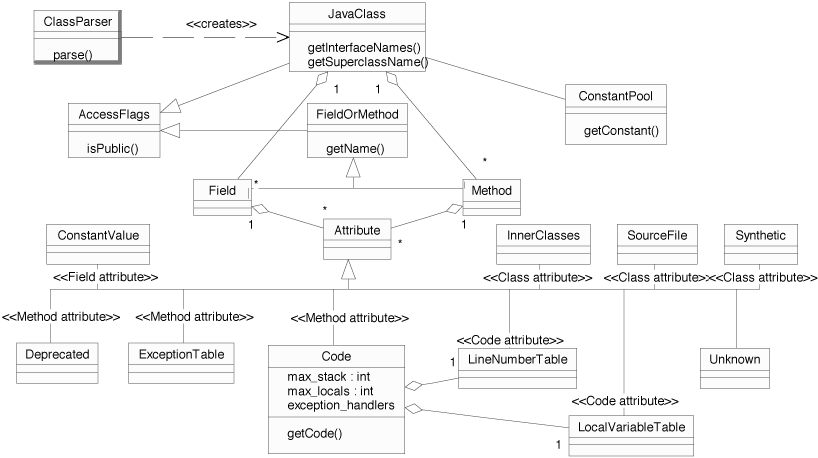
\includegraphics[width=28cm,height=16cm]{imagens/javaclassUML.png}
  \caption{diagrama de classe de BCEL \label{img:javaclassUML}}
\end{figure}

BCEL tamb�m � util na aprendizagem sobre a Java Virtual Machine (JVM) e o formato dos arquivos class. Compiladores, otimizadores, obfuscadores, geradores de c�digo e ferremantes de an�lise, vem utilizando BCEL com sucesso. Varios desses projetos podem ser consultados em http://jakarta.apache.org/bcel/projects.html.
Dada a exist�ncia de BCEL n�o foi necess�rio implementar um leitor de arquivos class, que � de suma import�ncia para o desenvolver desse trabalho. Necess�rio foi, aprender a trabalhar com as ferramentas e conhecer a API de BCEL.

\chapter{Id�ia base}
Atualmente a grande quantidade de biblietocas e frameworks para a linguagem Java facilitam e diminuem o tempo de desenvolvimento de aplica��es para esta linguagem. Parsers XML, frameworks de persisten�ncia, bibliotecas de logging, s�o exemplos de softwares j� desenvolvidos e testados que s�o utilizados em larga escala por outras aplica��es Java. No entanto estas bibliotecas e frameworks s�o projetadas para abrangerem a maior quantidade de situa��es que um desenvolvedor possa enfretar. Muitas vezes o desenvolvedor n�o utiliza todos os artif�cios que um bibliteca ou fgrameworks oferece, mas o c�digo que n�o � utlizado tamb�m � disponibilizado juntamente com a aplica��o final. Isso impacta na hora de usu�rio do aplicativo efetuar o download ou at� impossibilitando a instala��o da aplica��o por falta de espa�o no dispositivo, este �ltimo aspecto aplicasse a plataforma J2ME.
Como s� parte da biblioteca ou framework ser� necess�ria a aplica��o, a retirada da c�digo n�o utilizado diminuiria a tempo de download e apliaria a gama de dispositivos capazes de executar a aplica��o.
Uma analise est�tica do c�digo j� compilado da aplica��o, poder� nos fornecer as classes, m�todos e atributos que realmente fazem parte da aplica��o e a partir desses dados eliminar tudo que n�o vier a ser realmente utilizado na execu��o do software. Assim gerando um aplica��o equivalente, no entanto, menor.
� essa a finalidade do JMinimizer, eliminar tudo que n�o vier a ser utilizado na execu��o da apli��o.

\chapter{Implementa��o do Compactador de Aplica��es Java}

Um programa Java pode ter dois tipos de depend�ncia relacionados a bibliotecas e frameworks de terceiros. 
O primerio tipo de depend�ncia est� vinculado ao ambiente em que a aplica��o depois de pronta ser� executado, e nesse artigo a identificamos como depend�ncia do tipo \textit{runtime}. Suponhamos que estamos desenvolvendo um aplicativo para dispositivos m�veis com suporte a Wireless Message API. Estes dispositivos possuem implementa��es das classes do pacote javax.wireless.messaging, sendo assim estas classes j� estam disponiveis no ambiente de execu��o, no entanto para a compila��o e para a analise est�tica do c�digo elas s�o desconhecidas. Para a analise est�tica � preciso referencia-la, para que quando o JMinimizer come�ar a analiser a aplica��o ele encontre todas as classes e interfaces que s�o refer�ncidas no c�digo.
O outro tipo de depend�ncia n�o est� relacionado ao ambiente de execu��o, no entanto tamb�m deve estar presente neste. Esse tipo de depend�cia � criada pelo desenvolvedor quando para solucionar problemas de infra estrutura tipo parsers XML, logging, persist�ncia, este utiliza bibliotecas e/ou frameworks para resolve-los. Como esta depend�ncia n�o est� dispon�vel no ambiente de execu��o ela deve ser disponibilizada juntamente com a aplica��o. Aqui neste artigo a identificamos como depend�ncia do tipo \textit{program}.
Dito isto j� entedemos que as depend�ncias do tipo \textit{runtime} n�o precisam de nenhum tipo de tratamento, j� que elas fazem parte do ambiente de execu��o. J� as depend�ncias do tipo \textit{program} podem e devem ser modificadas para diminuir o tamanho final da aplica��o, j� que elas devem ser disponibilizadas juntamento com o software.

O arquivo de configura��o do JMinimizer possue sec��es para a devida declara��o de quais bibliotecas fazem parte da depend�ncia do tipo \textit{runtime} e do tipo \textit{program}. 

Exemplo de depend�cia do tipo \textit{program}.
\lstset{
      language=XML,
      basicstyle=\scriptsize,
      %labelstyle=\scriptsize,
      %labelsep=1pt,
      %labelstep=1,
      tabsize=2,
      %firstlabel=1
  }

\lstinputlisting{fontes/programClasspath.xml}

Tamb�m no arquivo de configura��o � necess�rio declarar o \textit{entry point} da aplica��o. Geralmente o \textit{entry point} � o m�todo main, startApp (para Midlets) ou start (para Applets). Al�m do m�todo \textit{entry point} tamb�m � necess�rio declarar os m�todos que ser�o chamados pelo ambiente de execu��o. Exemplo disto s�o os m�todos startApp, pauseApp e destroyApp de um Midlet.


\lstinputlisting{fontes/entryPoint.xml}

Existe a possibilidade tamb�m de declarar pontos de parada para o JMinimizer, suponhamos que n�o h� a necessidade de analisarmos classes do pacote \textbf{java.io}, basta para isso que declaremos no arquivo de configura��o o seguinte trecho.

\lstinputlisting{fontes/notInspect.xml}

Feito isso todas as invoca��es de m�todos de classes pertencentes ao pacote\textbf{java.io} n�o ser�o analisadas.
Tendo configurado as depend�ncias os m�todos que necessitam ser inspecionados e pontos de parada o JMinimizer ir� m�todo a m�todo declarado inspecionar seu c�digo a procura de novas invoca��es de m�todos e acesso a atributos, tanto est�ticos ou n�o. A medida que vai se achando novas invoca��es, essas chamadas de m�todos e/ou atributos s�o adicionadas, se n�o pertencerem a um padr�o de parada, � uma lista que cont�m uma �nica entrada para cada invoca��o de m�todo ou acesso � atributo. No final do processo esta lista conter� todos os m�todos e atributos que realmente compo�m o programa. Tanto m�todos concretos, abstratos e nativos s�o adicionados a est� lista, no entanto quando o JMinimizer encontra um m�todo abstrato ou nativo ele n�o far� a inspe��o do c�digo, obviamente por este n�o o possuir.
Durante este processo � verificado para cada novo m�todo encontrado se este representa \textit{\_java.lang.Class.forName(java.lang.String className)} se sim o m�todo que cont�m a invoca��o deste m�todo � adicionado a uma lista que ser� processada posteriormente e uma mensagem de alerta � enviada ao usu�rio informando-o que tal m�todo possui invoca��o de \textit{\_java.lang.Class.forName(java.lang.String className)}. Tudo isto � feito por que a linguagem Java suporta o carregamento din�mico de classes. Dito isto, � necess�rio, para uma correta analise e tranforma��o do c�digo, que o usu�rio declare no arquivo de configura��o todas as classes que eventualmente poder�o ser carregadas atrav�s da invoca��o do m�todo que cont�m a chamada � \textit{\_java.lang.Class.forName(java.lang.String className)}.
Finalizando o processo de analise, verificamos para todas as classes que foram encontradas, at� ent�o no processo, se estas classes possuem m�todos que foram sobre escritos de suas classes e/ou interfaces pais. Se estas possuem m�todos sobre escritos e que ainda n�o fazem parte da lista com todos os m�todos da aplica��o, estes ser�o adicionados a lista de m�todos ainda n�o processados e o processo recome�ar�. Ainda nessa etapa de analise � verificado para cada classe processada se est� possue a invoca��o do m�todo \textit{pacote.NomeDaClasse.$<$cinit$>$ ()V} que � o "construtor" padr�o da classe. Esse m�todo � invocado uma �nica vez ap�s o carregamento da classe pela JVM. Ele � utilizado para setar valores a vari�veis do tipo \textit{static final}.

O resultado dessa etapa de analise � uma lista, sem entradas repetidas, com todos os m�todos e campos que fazem realmente parte da aplica��o. A partir dessa lista e de uma segunda lista com todas a classes que est�o dispon�veis como depend�ncias do tipo \textit{program} ser� feita transforma��es visando a diminui��o do c�digo necess�rio para a execu��o da aplica��o. 
A classe que efetua a transforma��o implementa o padr�o \textit{Visitor}, assim sendo ela percorre� todas as classes que foram encontradas durante a etapa de analise e verificar� para cada uma delas se esta possue m�todos ou atributos que podem ser removidos. Se o m�todo ou campo  pode ser removido, ent�o ele � removido, caso contrario, e o m�todo perten�a a lista de m�todos que invocam \textit{\_java.lang.Class.forName(java.lang.String className)}, � feita uma verifica��o no seu c�digo para identificar se a chamada do m�todo  \textit{\_java.lang.Class.forName(java.lang.String className)} foi implementada pelo desenvolvedor ou se foi um artif�cio usado pelo compilador para transformar a constru��o: \texttt{Class number= Number.class} numa chamada ao m�todo  \textit{java.lang.Class.forName(java.lang.String className)}. Caso tenha sido o compilador que tenha produzido este c�digo duas a��es ser�o tomadas:
\begin{enumerate}
\item Ser� criado um m�todo, na classe corrente em analise, que ser� respons�vel unica e exclusivamente a carregar classes oriundas da constru��o \texttt{Class number= Number.class}. Este m�todo ter� acesso publico e est�tico com a finalidade de todas as classes da aplica��o terem acesso a ele. Esta a��o � tomada uma �nica vez. Ela ocorre na primeira vez que for encontrado um c�digo escrito pelo compilador com a finalidade de transformar em \textit{bytecode} a constru��o \texttt{Class number= Number.class}. Assim que a a��o se conclui o nome da classe em que foi adicionado o m�todo � armazenado para que o 2� passo seja executado sem problemas.
\item Ser� modificado o m�todo que invoca  \textit{\_java.lang.Class.forName(java.lang.String className)} para que a partir de agora ele invoque o m�todo que foi criado no passo anterior.
\end{enumerate}
O passo seguinte na transforma��o � retirar os atributos \textit{Deprecated, SourceFile, LineNumberTable, LocalVariableTable, Synthetic} das classes e ou interfaces e de seus membros (m�todos e campos), caso no arquivo de configura��o tenha sido declarado que deve ser feita uma compacta��o radical. A execu��o desse passo deve s� ser feita quando o software foi testado exaustivamente, tanto na sua forma original como na forma compactada, pois os atributos que foram removidos s�o utilizados para debugging e portanto a aplica��o deve estar est�vel para sofrer uma compacta��o radical.
Finalizando o processo temos a persist�ncia da classe compactada e de todos os arquivos que est�o dispon�veis no classpath da depend�ncia do tipo \textit{program} e que n�o s�o arquivos do tipo \textit{bytecode}, entre eles est�o arquivos XML, figuras, etc. O programa final pode ser persistido num diret�rio ou em um arquivo do tipo jar\cite{jar}, essa configura��o � feita no arquivo de configura��o do projeto.

\chapter{Estudo de caso}

Inicialmente o projeto teve como alvo a plataforma J2ME, subdividindo-se em perfis e configura��es. Contudo uma outra t�cnologia pode, facilmente, tirar proveito dos benef�cios que o JMinimizer pode trazer, essa t�cnologia � Applet. Applets s�o aplicativos Java que s�o executados dentro dos navegadores de Internet, eles s�o embutidos nas p�ginas HTML e quando o navegador encontra uma tag que indica a existencia de um Applet o navegador invoca uma m�quina virtual Java para interpretar e renderizar o Applet na p�gina HTML. Normalmente os applets s�o disponibilizados na forma de um arquivo jar {\LARGE colocar link para JAR}, e este pode ser relativamente grande e levar um tempo elevado para ser totalmente recebido pelo navegador que ir� renderiza-lo. A grande vantagem que o JMinimizer trar� neste caso � a diminui��o do tempo de recebimento do arquivo jar {\LARGE colocar link para JAR}, visto que computadores geralmente n�o possuem problemas de armazenamento.
Percebido isto, vi na t�cnologia applet um outro campo de utiliza��o do JMinimizer. E foi nesse outro campo que o JMinimizer foi utilizado primeiramente. 
Bem, como todo estudante de ci�ncias da computa��o que estuda e trabalha, eu tamb�m gosto de fazer alguns projetos tempor�rios e foi num desses projetos que eu vi uma oportunidade de experimentar o JMInimizer. O projeto era um site de encontros que possuiria um chat para que os assinantes pudessem se encontrar e conversar. O chat seria uma vers�o mais simples dos famosos Messeger e ICQ. A primeira vers�o realmente foi uma vers�o simples de seus inspiradores {\LARGE mostrar figura com a vers�o}.No entanto, os propriet�rios do site decidiram oferecer algo mais elaborado aos seus assinantes. Decidiram que o chat deveria oferecer op��es como trocar a cor da fonte das caixas de conversa��o e permitir que o usu�rio inserisse {\LARGE emoticons}, tudo isso nem perder compatibilidade com a vers�o 1.1 do Java, que era a vers�o que os sistemas operacionais Windows 2000 possuiam embutidas. Para tal esfor�o, foram encontradas duas solu��es iniciais: a primeira seria desenvolver o chat utilizando o framework de interface gr�fica chamado Thinlet, que propoe o desenvolvimento de interfaces gr�ficas baseadas em arquivos XML e � compativel com a vers�o 1.1 do Java. No entanto esse framework deixou a desejar quando comecei a tratar os eventos de teclado e por isso foi abandonado. A segunda op��o era utilizar swing, mas ela foi rapidamente descartada devido a n�o exist�ncia de tal pacote na vers�o 1.1 do Java.
A partir desse ponto iniciou-se uma pesquisa na Internet para que encontrasse um framework que suprisse nossa necessidade e tivesse compatibilidade com a vers�o 1.1 do Java. Com a ajuda dos sites de busca encontramos um projeto, antigo, mas que se encaixava perfeitamente nos requisitos que necessitavamos. Tal projeto � chamado de {\LARGE jp.kyasu}, e est� disponivel em http://openlab.jp/kyasu/, esse projeto � uma "reescrita" dos componentes do pacote \textit{java.awt} adicionando features que s� foram desenvolvidas futuramente para os componentes do pacote \textit{javax.swing}.
No entanto, o projeto � grande para ser obtido via internet, cerca de 626 kilobytes, principalmente se considerarmos as conex�es discadas. A partir desse momento encontrei uma grande chance de testar e aprimorar o JMinimizer.
Os primeiros testes com o applet se mostraram falhos, j� que a aplica��o n�o funcionava como deveria. Isso era gerado por diversos fatores que foram arrumados ao longo do desenvolvimento do JMInimizer. Em 21/05/2004 foi gerado uma vers�o est�vel que analisava e transformava com sucesso o chat e mais ainda diminuia sensivelmente o tamanho da aplica��o, tornando assim praticavel a distribui��o da mesma pela internet.

\begin{center}
 \begin{tabular}{|c|c|}
   \hline
	M�todo			&	bytes	\\
   \hline
	Sem transforma��o	&	719.692	\\
   \hline
	Com transforma��o	&	293.890	\\
   \hline
 \end{tabular}
\end{center}

\chapter{Trabalhos futuros}

Apesar de ter chegado � uma vers�o funcional e est�vel, ainda existem melhorias que podem ser adicionadas ao JMinimizer. A seguir est�o listadas, em ordem crescente de prioridade, as a��es que ser�o tomadas em rela��o ao projeto.

\section{Submeter artigo ao BYTECODE 2005}
Elaborar e submeter um artigo ao \textit{First Workshop on Bytecode Semantics, Verification, Analysis and Transformation}\cite{workshop} que ocorrer� em Edimburgo, Esc�cia no dia 9 de abril de 2005. 

\section{Integra��o a um obfuscador}
A integra��o com um obfuscador traria al�m de dificultar a engenharia reversa, uma diminui��o do c�digo final da aplica��o. Esse segundo aspecto � de grande import�ncia visto que o objetivo desse trabalho � mesmo diminuir o tamanho das aplica��es. Exposto isso fica claro que uma integra��o com um obfuscador aumentar� o percentual de compacta��o de uma aplica��o.

\section{Desenvolver um plugin para Maven}
Atualmente uma grande quantidade de aplicativos possuem integra��o ao Maven, e essa integra��o � feita atrav�s de plugins. Uma vers�o beta desse plugin para o JMinimizer j� esta em testes no entanto a falta de tempo paralizou seu desenvoilvimento.

\section{Ampliar as formas de declarar m�todos \textit{entry point}}
Nos primeiros testes com aplica��es reais surgiu a necessidade de declarar m�todos que devem ser analisados de uma forma diferente da que a usual, por exemplo por pacotes. Essa melhoria traria diminui��o no tempo de configura��o do JMinimizer.

\section{Compatibiliza��o com o J2SE 5.0}
Recentemente foi lan�ado a vers�o 5.0 da plataforma J2SE\footnote{Java 2 Standart Edition}, que traz entre outras coisas o recurso de Anota��es, que possibilita o desenvolvedor marcar m�todos e campos para que outras ferramentas possam identifica-los e processa-los facilmente. No entanto esse novo recurso de Java impactou na modifica��o da estrutura do bytecode, portanto a atual vers�o do JMinimizer e tamb�m BCEL � imcompat�vel com esta vers�o da plataforma. Assim que BCEL for compat�vel com a nova plataforma ser� iniciado um esfor�o para, tamb�m, compatibilizar o JMinimizer a plataforma 5.0 do J2SE. Como foi adquirido grande conhecimento da biblioteca BCEL, tanto nas ferramentas como at� mesmo no c�digo fonte, me disponibilizei para ajudar na compatibiliza��o do BCEL ao Java 5.0.

\section{Testar diferentes compiladores}
Atualmente os testes feitos com o JMinimizer foram realizados com o bytecode gerado por somente dois compiladores. O compilador fornecido pela Sun\cite{sun} e o compilador embutido na IDE Eclipse\cite{eclipse}. No entanto existem muitos compiladores para a linguagem Java e � de extrema necessidade que para todos os compiladores que um desenvolvedor possa utilizar que o JMinimizer analise e transforme o bytecode de forma correta. Para isso h� a necessidade de testar e homologar o JMinimizer com estes compiladores.

\section{Gera��o de relat�rios}
A gera��o de relat�rios � algo que est� parcialmente implementado, visto que a gera��o de arquivos XML com os m�todos e campos que s�o excluidos j� � feita. No entanto arquivos XML s�o de dif�cil interpreta��o por humanos. Arquivos PDF\footnote{Portable Document Format} e HTML\footnote{HyperText Mark-up Language} s�o de melhor entendimento e para a gera��o destes arquivos basta uma simples transforma��o de um arquivos XML com uma folha de estilo XSL\footnote{eXtensible Stylesheet Language}. 

\section{Desenvolver uma interface gr�fica}
O desenvolvimento de uma interface gr�fica para o JMinimizer tamb�m esta planejado para ser desenvolvido, no entanto sua prioridade � baixa. Na interface gr�fica seriam criados \textit{wizards} para configurar o JMinimizer, para gerar relat�rios em diversos formatos (PDF, HTML). A execu��o do JMinimizer tamb�m poderia ser feita atrav�s dessa interface, possibilitando at� uma barra de progresso indicando as etapas de execu��o do JMinimizer.

\chapter{Metodologia}
Desde que comecei a trabalhar como desenvolvedor Java, tive contato com in�meros projetos \textit{open-source}\footnote{do ingl�s c�digo-aberto} e dentre estes observei que alguns utilizavam a m�todologia de desenvolvimento de software chamada de XP\footnote{eXtreme Programming}, que me chamou a aten��o. Como nunca havia desenvolvido software baseado nessa metodologia, resolvi aplica-la, no desenvolvimento do JMinimizer. � claro que n�o consegui ser um extremista e seguir ao p� da letra o que XP recomenda, mas algumas pr�ticas que achei interessante adotei no desenvolvimento desse trabalho, entre elas est�o: a confec��o de testes unit�rios e a libera��o de vers�es num per�odo menor. A cria��o de testes unit�rios mostrou ser de grande import�ncia nas etapas de desenvolvimento, principalmente quando as altera��es no c�digo fonte eram profundas, pois terminada as altera��es eram executados os testes unit�rios e validados ou n�o as altera��es feitas. J� a libera��o de vers�es num per�odo menor foi pouco utilizado, pois como n�o haviam "clientes" esperando pelo software n�o foi preciso liberar vers�es, no entanto quando foi obtido uma vers�o est�vel do JMinimizer, foram gerados marcos no controlador de vers�o do projeto, para que posteriormente essas vers�es est�veis pudessem ser obtidas, mesmo depois de alterados os c�digos fontes do programa.
Tamb�m inspirado nos projeos \textit{open-source} e na minha vida profissional adotei ferramentas de desenvolvimento que se tornaram padr�es na confec��o de aplica��es Java. Dentre todas, 6 programas foram essenciais. Inicando pelo sistema operacinal \textit{Fedora Core 1 e 2}\cite{fedora}, que � uma distribui��o do sistema operacional Linux. O conjunto de ferramentas distribu�das pela Sun\cite{sun} para desenvolvimento de aplica��es Java chamando de J2SE SDK\footnote{Software Development Kit} tamb�m foi utilizado nas suas vers�es 1.4.2\_02 e 1.4.2\_4. A IDE\footnote{Integrated Development Environment} Eclipse\cite{eclipse} foi o ambiente de desenvolvimento utilizado para criar o JMinimizer, seu compilador embutido para Java tamb�m foi instrumento de uso dessa tese. O controlador de vers�o CVS\footnote{Concurrent Versions System}\cite{cvs}, foi utilizado para manter de forma organizada as vers�es que eram geradas dia ap�s dia do c�digo fonte da aplica��o. A vers�o 1.11.1p1 foi utilizado no servidor do CVS e as vers�o 1.11.15, 1.11.16 e 1.11.17 no cliente. Integrando todas essas ferramentas foi utilizado o Maven \cite{maven} para gerenciar o projeto. Tarefas como compilar, executar os testes unit�rios, gerar documenta��o, m�tricas, relat�rios, criar artefatos, gereciar o controlador de vers�o eram executadas atrav�s da ferramenta Maven que prov� uma interface �nica para execu��o de todas essas tarefas.



\chapter{Conclus�o}
O desenvolvimento de aplica��es baseadas em bibliotecas de terceiros � ivariavelmente uma solu��o inteligente quando n�o queremos ou podemos desenvolver infra estrutura para nossa aplica��o. E com a ajuda do JMinimizer 






\renewcommand\bibname{Refer�ncias Bibliogr�ficas}
\bibliographystyle{abnt} % Estilo para gerar refer�ncias em conformidade com
                         % as normas brasileiras
\bibliography{tcc}

\end{document}
